\documentclass[10pt,twocolumn]{article}

% ---------------------------------------------------------------------------
%  Waggle: Name Semantics for Agent Handoffs
%  A systems paper. Classic two-column, Computer Modern, hand-drawn TikZ.
% ---------------------------------------------------------------------------

\usepackage[T1]{fontenc}
\usepackage{lmodern}
\usepackage[utf8]{inputenc}
\usepackage[hmargin=1.85cm,vmargin=2.1cm,columnsep=0.7cm]{geometry}
\usepackage{microtype}
\usepackage{booktabs}
\usepackage{array}
\usepackage{amsmath,amssymb}
\usepackage{tikz}
\usetikzlibrary{arrows.meta,positioning,calc,fit,backgrounds,shapes.geometric,decorations.pathreplacing}
\usepackage{pgfplots}
\pgfplotsset{compat=1.18}
\usepackage[ruled,vlined]{algorithm2e}
\usepackage{caption}
\usepackage{enumitem}
\usepackage[hidelinks]{hyperref}
\usepackage[numbers,sort&compress]{natbib}
\usepackage{balance}

\captionsetup{font=small,labelfont=bf}
\setlist{nosep,leftmargin=1.2em}
\SetKwComment{Comment}{$\triangleright$\ }{}
\newcommand{\tok}[1]{\texttt{#1}}
\renewcommand{\ttdefault}{cmtt}

% Consistent muted palette (prints legibly in greyscale).
\definecolor{ink}{HTML}{1A1A1A}
\definecolor{stone}{HTML}{6B6B6B}
\definecolor{pale}{HTML}{EDEDE8}
\definecolor{line}{HTML}{4A4A4A}

\title{\vspace{-1.2em}\textbf{The Dance and the Field:\\[2pt]
Name Semantics for Handoffs Between Distributed Agents}}

\author{
  Chetan Conikee\\
  \normalsize Modiqo\\
  \normalsize\texttt{chetan@modiqo.ai}
}
\date{}

\begin{document}
\maketitle

\begin{abstract}
\noindent
Agent harnesses are becoming distributed systems: a single task now fans
out across dozens of subagents, within one process, across the harnesses
on a machine, and increasingly over the network. Yet the mechanism these
systems use to pass work between agents is the one that distributed
systems abandoned decades ago---\emph{copy the bytes and hope}. A report
produced by one agent is pasted into the context of the next, re-billed
on every subsequent turn of a stateless API, duplicated across every
recipient, and stripped of identity, version, and any record of whether
it was read. Copies are the root defect: a copy has no owner, no
lifecycle, and no receipt, and roughly a third of multi-agent failures
trace to agents acting on divergent copies of what should have been the
same information.

We present \textsc{waggle}, a substrate built on \emph{name semantics}.
A handoff is a $\sim$30-byte attributed token, not a payload. Consumers
do not receive content; they \emph{resolve} the token into a projection
computed for their own context, \emph{interrogate} it under byte budgets
where the bytes live, and leave \emph{receipts} in an append-only,
payload-free log. The same five verbs operate unchanged at three
radii---inter-process, inter-harness, and inter-machine---which is the
paper's central systems argument: portability of a handoff cannot be an
optimization applied to copies; it must be a property of the reference.
We ground the design in a lineage the agent literature has overlooked:
tuple spaces, named-data networking, capabilities, leases, and
stigmergy. We describe a sealed context-adaptive matcher, a
consumption-contract mechanism that turns ``did the subagent actually
read it?'' from an unanswerable question into a query, and a mint-time
structural lens for source code that gives an agent a symbol-addressable
handoff without any parser on the serving path. We report microbenchmarks
(39\,ns cache-hit resolution, 323\,\textmu{}s end-to-end over a domain
socket, a million-event fold in 334\,\textmu{}s) and a live delegation
case study, and we are candid about the mechanism's limits.
\end{abstract}

% ===========================================================================
\section{Introduction}
% ===========================================================================

Begin with the fact that shapes everything else: large-language-model
APIs are \emph{stateless}. Each turn of a conversation re-sends the entire
conversation. When an agent places a 40\,KB report into its context, it
does not pay for that report once; it pays on every subsequent turn of
that agent's life, because the whole history rides along each time. Now
add a second agent. An orchestrator receives a report and forwards it to
a writer subagent; the report now occupies \emph{two} context windows,
each re-billing it per turn. Add a fact-checker: three. This is not a
defect of any one framework---it is the default shape of the ecosystem.
LangGraph's handoff tool ``by default passes the full message
history''~\citep{langgraph}; Anthropic, engineering their own multi-agent
research system, measured agents at ${\sim}4\times$ the tokens of chat and
multi-agent systems at ${\sim}15\times$, attributing the overhead to
``duplicating context across agents'' and writing the sentence this work
is built on: \emph{``each handoff loses context''}~\citep{anthropic2025}.
The MAST failure taxonomy attributes \textbf{36.9\%} of multi-agent
failures to inter-agent misalignment---agents acting on divergent, stale,
or partial copies of what should have been the same
information~\citep{cemri2025}.

Copies are the root defect. A copy has no identity, no version, no owner,
no lifecycle. The moment the author corrects the report, every pasted copy
is silently wrong, and no mechanism exists to find them. The token cost is
what everyone feels; the missing lineage and the impossibility of
correction are what actually break swarms.

\paragraph{Thesis.} Passing work between computational actors admits
exactly three disciplines. \emph{Copy semantics} (message passing) sends
the bytes---simple, and every pathology above follows. \emph{Place
semantics} (shared memory) has both parties touch one location---this
fixes duplication but demands shared infrastructure and says nothing about
who may see what. \emph{Name semantics} sends a small, immutable,
attributed \emph{claim} and lets resolution be computed per consumer, at
the data, on demand. Distributed systems learned to prefer the third
discipline for exactly the reasons agent systems are now
rediscovering. This paper argues that the agent handoff is a
distributed-systems problem, that name semantics is its right shape, and
that a substrate built on names makes a handoff behave identically whether
its two ends sit in one process or on two continents. We substantiate the
argument with a working system, \textsc{waggle}~\citep{waggle2026}, and
its measurements.

\paragraph{Contributions.}
\begin{itemize}
  \item A framing of agent handoffs as a distributed-systems problem, with
    a four-boundary analysis (\S\ref{sec:problem}) showing that every
    boundary loses lineage and cannot propagate corrections.
  \item A substrate for \emph{name semantics} (\S\ref{sec:design}): a
    30-byte attributed token, a three-zone signed manifest, a sealed
    context-adaptive matcher (Alg.~\ref{alg:match}), and an append-only
    payload-free log with an exact-reconstruction guarantee.
  \item \emph{Receipts} (\S\ref{sec:receipts}): consumption contracts and
    a coverage fold (Alg.~\ref{alg:coverage}) that make delegated
    consumption verifiable without trusting the consumer's self-report.
  \item A \emph{structural lens} for source code (\S\ref{sec:lens})
    computed once at mint, so no parser ever runs on a serving path---%
    including the network edge.
  \item The \emph{three-radii} result (\S\ref{sec:radii}): the identical
    verb loop inter-process, inter-harness, and inter-machine.
  \item An evaluation (\S\ref{sec:eval}) of microbenchmarks and a live
    delegation, an honest comparison against lexical search, and a frank
    account of limits (\S\ref{sec:limits}).
\end{itemize}

% ===========================================================================
\section{The Handoff Problem}
\label{sec:problem}
% ===========================================================================

``Passing a resource between agents'' is four different problems wearing
one name, distinguished by which boundary the resource crosses.
Table~\ref{tab:boundaries} reads, column by column, as a ledger of what is
lost. The two rightmost columns are empty top to bottom: no boundary today
carries lineage, and none propagates a correction. That emptiness is the
problem this paper attacks.

\begin{table*}[t]
\centering
\small
\caption{The four boundaries of an agent handoff. Read the last two
columns top to bottom: they are empty. Lineage and correction do not
survive any boundary today.}
\label{tab:boundaries}
\renewcommand{\arraystretch}{1.25}
\begin{tabular}{@{}p{2.9cm}p{4.1cm}p{4.1cm}p{2.4cm}p{2.0cm}@{}}
\toprule
\textbf{Boundary} & \textbf{How it works today} & \textbf{What travels} &
\textbf{Lineage} & \textbf{Corrections}\\
\midrule
Same harness, same model (orchestrator $\to$ subagent) &
Final message returns to the orchestrator, which pastes what the next
subagent needs; or shared filesystem paths by convention &
The full text again, per recipient; a path travels cheaply but carries no
version, access story, or receipt &
None---prose memory, gone at compaction &
Manual re-paste; stale copies persist silently\\
Same harness, mixed models (router / cascade) &
The same paste, now crossing a billing boundary &
The full text, re-tokenized under a different tokenizer &
None &
None\\
Across harnesses, one machine &
Files on disk plus convention files, or a human copy-pastes between panes &
A path with no semantics, or the text itself &
None---the filesystem records mtime, not meaning &
None---delete the file and one side breaks silently\\
Across machines / orgs &
Chat, email, tickets, shared drives; artifact-by-URL at the frontier &
Whole artifacts, or URLs whose resolution semantics no standard defines &
Whatever the messaging tool retains, divorced from the artifact &
Effectively impossible\\
\bottomrule
\end{tabular}
\end{table*}

\paragraph{Why provider optimizations do not save you.} Every vendor is
attacking the token cost inside its own walls: prompt caching discounts
byte-identical prefixes within a short TTL and a single account; harness
compaction summarizes a long context locally and lossily. These are real
savings. But each is scoped to one vendor's billing and serving boundary.
A cached prefix at one provider means nothing at another's tokenizer; a
compaction summary in one harness does not exist in another. Cross any row
of Table~\ref{tab:boundaries} and you pay full freight again, because what
crossed was a copy of bytes, and bytes carry no identity a foreign system
could recognize. This is the structural case for name semantics:
portability cannot be an optimization applied to copies. It must be a
property of the reference. A 30-byte token is the same 30 bytes in every
context window, every tokenizer, every vendor, every machine; what varies
is what it \emph{resolves to}, computed fresh, per consumer, where the
bytes live.

% ===========================================================================
\section{What the Colony Knew}
\label{sec:bees}
% ===========================================================================

A honeybee returns from a field two kilometres out carrying information
worth sharing: where, how far, how good. She does not carry the field
home, nor enough nectar for the colony to evaluate. She
\emph{dances}~\citep{vonfrisch1967}. The waggle run's angle against
vertical encodes direction relative to the sun; its duration encodes
distance; its vigour encodes quality. Then the colony does something every
distributed-systems engineer should study: each follower resolves the
reference \emph{herself}---flies her own flight, with her own senses, from
her own position. The dance is not the nectar; it is an attributed,
resolvable claim that the nectar exists. Recruitment is measurable, one can
count who followed and who returned to dance in turn, and the information
expires honestly: bees dance only while the source still pays, so no bee
chases stale copies of yesterday's directions, because there were never
any copies to chase.

This is \emph{stigmergy}: coordination through durable marks rather than
direct messages~\citep{grasse1959,theraulaz1999}. The mapping to a handoff
substrate is structural, not decorative (Table~\ref{tab:mapping}). The
colony solved the multi-agent handoff problem with zero shared context
windows: share names, not payloads; let each consumer resolve per its own
capability; make consumption observable; let stale claims die at the
source.

\begin{table}[t]
\centering
\small
\caption{The dance and the substrate. The correspondence is structural.}
\label{tab:mapping}
\renewcommand{\arraystretch}{1.2}
\begin{tabular}{@{}p{3.7cm}p{4.0cm}@{}}
\toprule
\textbf{The dance} & \textbf{The substrate}\\
\midrule
Figure-eight encodes a vector in seconds & 30-byte token names an artifact plus its attribution\\
Each follower flies her own flight & Each consumer resolves \emph{its} projection (sealed matcher)\\
The follower's senses at the field & \tok{read}/\tok{search}: interrogate content on arrival\\
Countable recruitment & The funnel: resolve $\to$ read $\to$ run, as receipts\\
Dancers recruiting dancers & Lineage: children minted under parents\\
Dancing stops when nectar stops & Leases, supersession, revocation\\
The dance floor & The append-only log every mark lands on\\
\bottomrule
\end{tabular}
\end{table}

% ===========================================================================
\section{Design: Name Semantics}
\label{sec:design}
% ===========================================================================

\subsection{The token and the manifest}
A \emph{token} is 4--23 characters of Bitcoin base58 (default 8 public, 16
for private capability URLs), generated by rejection sampling to avoid
modulo bias. It is the same 30 bytes in every tokenizer. Behind it stands
an \emph{attribution manifest} in three zones with three mutability rules,
a separation that is load-bearing:

\begin{description}[leftmargin=1.1em,style=nextline]
  \item[Immutable core] set at mint, never changed: schema, token, target,
    sharer, channel, mint time, snapshot metadata, parent, the
    content-addressed snapshot reference, variants, and---optionally---a
    consumption contract (\S\ref{sec:receipts}) and a symbol-outline
    reference (\S\ref{sec:lens}). Signatures cover exactly this zone.
  \item[Versioned mutable] compare-and-swap by version: expiry,
    revocation, supersession. Every lifecycle change cites the version it
    was decided against.
  \item[Cosmetic mutable] last-writer-wins: campaign and labels.
\end{description}

Because signatures (Ed25519 over the canonical core bytes) cover only the
immutable zone, lifecycle and cosmetic churn never invalidate a
signature---the three-zone design's payoff, and a direct descendant of
capability discipline~\citep{dennis1966,miller2006}. Content over 64\,KiB
rides as a content-addressed reference~\citep{merkle1987,benet2014} rather
than inline, so the manifest stays small and the bytes stay verifiable
wherever they replicate.

\subsection{The sealed matcher}
A manifest carries one or more \emph{variants}, each a projection of the
artifact for a class of consumers, guarded by a match expression over four
dimensions: model family, harness, modalities, and posture. Selection is
\emph{sealed}: the algorithm is fixed and exposes no hooks, so the trust
claim ``the same context always receives the same projection'' survives
(Alg.~\ref{alg:match}). This is the resolve-per-consumer discipline of the
dance made deterministic: one name, many truthful renderings---a
Claude-tuned digest, an image for a vision agent, a transcript for an
agent without ears, fail-closed instructions for CI.

\begin{algorithm}[t]
\small
\caption{Sealed variant selection. Total over any manifest (mint
guarantees exactly one catch-all).}
\label{alg:match}
\DontPrintSemicolon
\KwIn{variants $V$; resolver context $c$}
\KwOut{index of the selected variant}
$best \leftarrow \bot$;\quad $bestSpec \leftarrow -1$\;
\For{$i \leftarrow 0$ \KwTo $|V|-1$}{
  \If{$\neg\, \textsc{Accepts}(V[i].expr, c)$}{\textbf{continue}\;}
  $s \leftarrow \textsc{Specificity}(V[i].expr)$
    \Comment*[r]{constrained dims, $0..4$}
  \If{$s > bestSpec$}{
    $best \leftarrow i$;\quad $bestSpec \leftarrow s$
      \Comment*[r]{ties: earlier declaration wins}
  }
}
\Return $best$\;
\BlankLine
\textbf{\textsc{Accepts}}$(e, c)$: every constrained dimension of $e$
admits $c$; an undeclared context value \emph{fails} a constrained
dimension; modalities match by superset.\;
\end{algorithm}

\subsection{The log is the truth}
Everything downstream of a mint is an \emph{event} in an append-only log,
and every view---manifest tables, funnel counts, lineage---is a fold over
that log~\citep{kreps2013}. Two invariants make the log safe to replicate
anywhere. First, events are \emph{payload-free by construction}: the event
type is exactly $\langle \textit{token}, \textit{stage}, \textit{actor},
\textit{time}, \textit{seq}, \textit{variant?}, \textit{regions?}\rangle$,
and no payload field \emph{exists}, so the receipt trail can never become
the leak. The actor is a coarse class---kind, model family, harness
class---never a version or an instance identifier. Second, reconstruction
is exact: folding the log rebuilds byte-identical state regardless of
arrival order, and is immune to duplicate and shuffled records
(Fig.~\ref{fig:log}). Migration is therefore a \emph{stream}: export the
log, replay it elsewhere, and the destination \emph{is} the source---same
tokens, same history, same receipts. This is the property that makes
``across machines'' transport plus replication rather than new
architecture.

\begin{figure}[t]
\centering
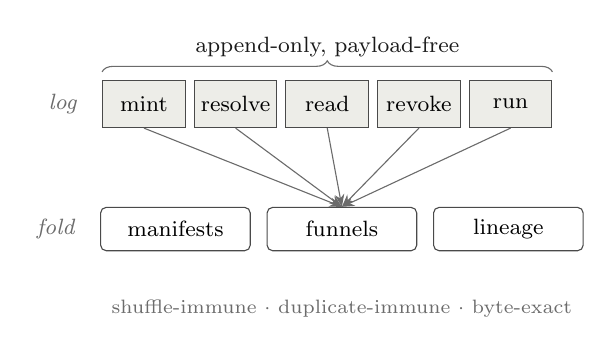
\begin{tikzpicture}[
  font=\footnotesize,
  rec/.style={draw=line,fill=pale,minimum width=1.05cm,minimum height=0.6cm,inner sep=1pt},
  view/.style={draw=line,rounded corners=2pt,minimum width=1.9cm,minimum height=0.55cm,inner sep=1pt},
  >={Stealth[length=1.6mm]}
]
% the log
\node[rec] (m) at (0,0) {mint};
\node[rec,right=1mm of m] (e1) {resolve};
\node[rec,right=1mm of e1] (e2) {read};
\node[rec,right=1mm of e2] (mu) {revoke};
\node[rec,right=1mm of mu] (e3) {run};
\node[left=2mm of m,text=stone] {\itshape log};
\draw[decorate,decoration={brace,amplitude=4pt},stone]
  ($(m.north west)+(0,1mm)$) -- ($(e3.north east)+(0,1mm)$)
  node[midway,above=2pt,text=ink]{append-only, payload-free};
% the fold
\node[view,below=1.0cm of m,xshift=0.4cm] (f1) {manifests};
\node[view,right=2mm of f1] (f2) {funnels};
\node[view,right=2mm of f2] (f3) {lineage};
\node[left=2mm of f1,text=stone] {\itshape fold};
\foreach \x in {m,e1,e2,mu,e3}{
  \draw[->,stone] (\x.south) -- ($(f2.north)+(0,0)$);
}
\node[below=0.5cm of f2,text=stone,align=center]
  {\scriptsize shuffle-immune $\cdot$ duplicate-immune $\cdot$ byte-exact};
\end{tikzpicture}
\caption{The log is the truth; every view is a fold. Reconstruction is
order-insensitive, so the log replicates freely and migration is a
replay.}
\label{fig:log}
\end{figure}

\subsection{Interrogation, not transmission}
The consumer's first move is never a blind fetch. Holding a token affords
three instruments, all under one hard byte-budget contract (default
4\,KB): \tok{query} slices the \emph{metadata} by pointer; \tok{read}
slices the \emph{content}---a line window, a named section, a code symbol,
a JSON path; \tok{search} greps the content and returns matches with full
counts even when the list is truncated. Every response names the bytes it
spared you, and carries executable ``next'' steps so an agent that only
follows guidance still reaches every leaf. Retrieval becomes
interrogation: a consumer that needs three facts from a sixty-page report
ingests a few hundred bytes, ever---the follower's senses at the field,
not the field carried home. This is a direct instance of the end-to-end
argument~\citep{saltzer1984}: the substrate moves the question to the data
rather than the data to the question, and the marginal-value calculus of
when to stop reading is the forager's~\citep{charnov1976,pirolli1999}.

% ===========================================================================
\section{Receipts: Verification Without Trust}
\label{sec:receipts}
% ===========================================================================

The orchestrator's real question about a delegation is not ``what did the
subagent say'' but ``did it actually read what I gave it.'' Under copy
semantics this is unanswerable; under name semantics it is a query. Every
resolve, read, and search is an event, so the \emph{funnel}---stage counts
per token, with actor classes, never payloads---reports which handoffs were
consumed, which stalled, and which delivered.

Two mechanisms sharpen a raw count into a verdict. A \emph{consumption
contract}, declared at mint and signed into the immutable core, names the
regions a consumer must reach (up to eight line ranges, or a threshold
fraction of them). At serve time, when a \tok{read} window or a
\tok{search} hit overlaps a required region, the serving path stamps a
\emph{manifest-referencing bitmask}---an index into the signed
declaration, never bytes---onto the event, preserving the payload-free
invariant exactly as the variant field does. A \emph{coverage} fold then
$\mathrm{OR}$s these bitmasks and reports met/unmet with the untouched
regions \emph{named} (Alg.~\ref{alg:coverage}); because $\mathrm{OR}$ is
commutative and idempotent, the fold inherits the log's shuffle- and
duplicate-immunity for free. Finally, the judge's verdict rides as its own
stages---\tok{accepted}, \tok{rejected}---so the outcome is derivable from
counts (pending / accepted / rejected / contested) and a rejection's
response teaches the escalation: re-mint the same target under the same
parent for a stronger consumer, then supersede the rejected child, so the
escalation itself becomes lineage.

\begin{algorithm}[t]
\small
\caption{Contract coverage. A pure fold; misses are named, never
silent.}
\label{alg:coverage}
\DontPrintSemicolon
\KwIn{token $t$; its contract regions $R$ (up to 8); its events $E$}
\KwOut{$met$; the list of untouched regions}
$bits \leftarrow 0$\;
\ForEach{$e \in E$ \textbf{with} $e.token = t$}{
  \If{$e.regions \neq \bot$}{$bits \leftarrow bits \mathbin{|} e.regions$
    \Comment*[r]{OR: order- and dup-immune}}
}
$touched \leftarrow \textsc{PopCount}(bits)$\;
$permille \leftarrow \lfloor 1000 \cdot touched / |R| \rfloor$\;
$met \leftarrow permille \geq R.threshold$\;
$missed \leftarrow \{\, R[i] : \text{bit } i \text{ of } bits = 0 \,\}$\;
\Return $(met, missed)$\;
\end{algorithm}

This is precisely the telemetry loop that skill authors and model vendors
lack today. It is also, deliberately, a proof of \emph{consumption}, not
of comprehension---a distinction we return to in \S\ref{sec:limits}. The
signal it produces is the raw material for post-hoc, evidence-based model
routing, a complement to the pre-hoc, prompt-feature routers of current
practice~\citep{ong2024}, and its interrogation traces are the kind of
step-level process-supervision data that improves
reasoners~\citep{lightman2023,jin2025} and lets successful trajectories be
distilled into scaffolds for weaker consumers~\citep{wang2024awm}.

% ===========================================================================
\section{A Structural Lens for Code}
\label{sec:lens}
% ===========================================================================

Source code is the handoff the substrate must serve well, because it is
what orchestrators most often delegate. Text tools---line windows and
regular-expression search---treat a program as a string. An agent handed a
code token instead wants to know \emph{what the file is} before it greps:
its functions, methods, and types, with line ranges. We compute that
structure once, at mint, where the artifact is at hand, using an
incremental parser~\citep{treesitter} and its tag queries, and store the
result---a flat, document-ordered outline of definitions---as a
content-addressed blob beside the snapshot.

The design decision that matters is \emph{where parsing happens}. It
happens only at mint, on the machine that owns the bytes. Serving the
outline is a blob fetch and a budget-fitted render---no parser on any
serving path, and in particular none at the network edge, whose runtime
could not host a native parser in any case. The outline is thus authored
content derived from pinned bytes: a pure function of the snapshot and an
extractor version, so it is minted once and never invalidated, and
identical bytes deduplicate for free. A \tok{read} by symbol name resolves
to the definition's exact line range through the ordinary windowed-read
path, so contract stamping applies unchanged; a \tok{require symbol:$N$}
requirement resolves the symbol to a line range at mint and enters the
signed contract. The lens does for code what section headings do for
prose, uniformly across languages, without a single new invariant.
Extraction is measured at 2.3\,ms per thousand lines
(\S\ref{sec:eval})---amortized entirely into the one-time mint.

% ===========================================================================
\section{One Loop at Three Radii}
\label{sec:radii}
% ===========================================================================

The systems claim of the paper is that a handoff behaves identically
regardless of the distance between its two ends. A single daemon owns the
local store; every harness on a machine speaks to it over a
filesystem-permissioned domain socket, so cross-harness handoff on one box
is not a feature but the default. Daemons federate to one another over
authenticated transport; the same tokens graduate to a network edge by
replaying the log, with content-addressed snapshots replicated so that a
\tok{search} runs \emph{at the edge} against content whose source file
never left the author's laptop (Fig.~\ref{fig:radii}). Because the shim
between a harness and the daemon adds no semantics---it pumps
JSON-RPC frames between a pipe and a socket---``across machines'' is
transport plus replication, not new architecture. An agent's loop---mint,
hand off one line, resolve, interrogate, report---is byte-for-byte the same
at all three radii. That invariance is the dividend of name semantics, and
it is why we claim distributed subagents are the near future rather than a
special case: the programming model does not change as the swarm spreads
from one core to many machines. The lineage here is old and deep---tuple
spaces made coordination a property of a shared
medium~\citep{gelernter1985}; named-data networking made the network route
by name rather than by host~\citep{jacobson2009}; leases made freshness a
bounded promise rather than a cache guess~\citep{gray1989}. \textsc{waggle}
is these ideas applied to the artifact a swarm of agents passes around.

\begin{figure}[t]
\centering
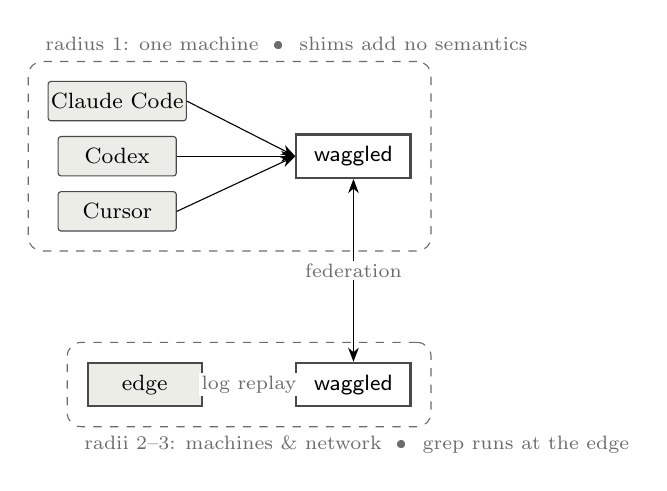
\begin{tikzpicture}[
  font=\footnotesize,
  >={Stealth[length=1.8mm]},
  proc/.style={draw=line,fill=pale,rounded corners=1pt,minimum width=1.5cm,minimum height=0.5cm,inner sep=1pt},
  dmn/.style={draw=line,thick,minimum width=1.45cm,minimum height=0.55cm,inner sep=2pt},
  radius/.style={draw=stone,dashed,rounded corners=5pt,inner sep=7pt}
]
% --- radius 1: one machine (top) -----------------------------------------
\node[proc] (h1) at (0,1.05) {Claude Code};
\node[proc] (h2) at (0,0.35) {Codex};
\node[proc] (h3) at (0,-0.35) {Cursor};
\node[dmn] (d1) at (3.0,0.35) {\textsf{waggled}};
\foreach \h in {h1,h2,h3}{\draw[->] (\h.east) -- (d1.west);}
\begin{scope}[on background layer]
\node[radius,fit=(h1)(h3)(d1)] (r1) {};
\end{scope}
\node[text=stone,font=\scriptsize,anchor=west] at ($(r1.north west)+(0.1,0.22)$)
  {radius 1: one machine \ \textbullet\ \ shims add no semantics};
% --- radii 2--3: machines & network (bottom) -----------------------------
\node[dmn] (d2) at (3.0,-2.55) {\textsf{waggled}};
\node[dmn,fill=pale] (edge) at (0.35,-2.55) {edge};
\draw[<->] (d1.south) -- (d2.north)
  node[midway,fill=white,inner sep=1pt,text=stone,font=\scriptsize]{federation};
\draw[<->] (edge.east) -- (d2.west)
  node[midway,fill=white,inner sep=1pt,text=stone,font=\scriptsize]{log replay};
\begin{scope}[on background layer]
\node[radius,fit=(edge)(d2)] (r2) {};
\end{scope}
\node[text=stone,font=\scriptsize,anchor=west] at ($(r2.south west)+(0.1,-0.22)$)
  {radii 2--3: machines \& network \ \textbullet\ \ grep runs at the edge};
\end{tikzpicture}
\caption{One token at three radii. The verb loop is identical; only the
transport lengthens. Computation travels to the data, so the edge answers
\tok{search} against snapshots whose source files never left the author's
machine.}
\label{fig:radii}
\end{figure}

Consumption is protocol-shaped rather than SDK-shaped: the substrate is a
Model Context Protocol server~\citep{mcp2024}, one configuration line in
any MCP-speaking harness. The interrogation verbs are exposed as
\emph{tools} because the protocol assigns model-controlled actions to
tools; the passive faces of a token---enumeration, plain read, and
subscription to lifecycle updates---are exposed as \emph{resources}, so a
correction propagates to holders as a protocol-native push. The frontier's
agent-to-agent efforts standardize artifact-by-URL and stop
there~\citep{a2a2025}; name semantics is the resolution discipline that
gap wants.

% ===========================================================================
\section{Evaluation}
\label{sec:eval}
% ===========================================================================

We evaluate three questions: is the reference cheap enough to prefer over
a copy; does verification-without-trust work on a real delegation; and how
does interrogation-through-a-token compare with the lexical search agents
use today.

\subsection{Microbenchmarks}
Table~\ref{tab:perf} reports the hot paths. Measurements are taken on
commodity hardware with a warm store; the domain-socket figure is
end-to-end through the shim, daemon dispatch, sealed match, event append,
and reply. The cache-hit resolution at 39\,ns and the million-event fold
at 334\,\textmu{}s establish that neither resolution nor the receipt
machinery is a bottleneck; the 323\,\textmu{}s socket round-trip is
dominated by the durable append's \texttt{fsync}, which is the price of the
$C\!$-1 durability guarantee, not of the abstraction. Symbol extraction at
2.3\,ms/kLOC is paid once, at mint.

\begin{table}[t]
\centering
\small
\caption{Hot-path measurements. The abstraction is not the cost; durable
persistence is.}
\label{tab:perf}
\renewcommand{\arraystretch}{1.15}
\begin{tabular}{@{}lr@{}}
\toprule
\textbf{Operation} & \textbf{Latency}\\
\midrule
Cache-hit resolution (sealed match + stamp) & 39\,ns\\
End-to-end resolve over domain socket (p50) & 323\,\textmu{}s\\
Durable event append (real \texttt{fsync}) & 39\,\textmu{}s\\
Million-event funnel fold & 334\,\textmu{}s\\
Symbol extraction (per 1000 lines, one core) & 2.3\,ms\\
Outline render under 4\,KB budget & ${\sim}0.1$\,ms\\
Edge resolve, full HTTP--worker path (p50) & 1.2\,ms\\
\bottomrule
\end{tabular}
\end{table}

\paragraph{The cost, measured.} Table~\ref{tab:cost} prices the same
delegation three ways against a deliberately strong baseline---a copy that
enjoys within-vendor prompt caching---and Figure~\ref{fig:cost} sweeps
artifact size at the five-consumer, five-turn operating point. Two
properties keep the account honest. The baseline is \emph{cached}, not the
straw-man of naïve re-sending; and the reported ratio is
\emph{tokenizer-invariant}---the tokenizer cancels in a ratio---so the
headline does not turn on a choice of BPE. The figure carries one central
fact: waggle's cost is \emph{flat in artifact size}, because the 30-byte
line and the bounded projection do not grow with the report, while the copy
grows linearly; the ratio therefore widens without bound, from
$2\times$ on a single-shot 4\,KB hand-off, through $44\times$ at the
40\,KB/five-consumer/five-turn cell, to $329\times$ under deep delegation.
We are equally plain about the floor: at $H{=}T{=}1$ the advantage is only
$2\times$, and the substrate earns its keep when an artifact is
\emph{shared or revisited}, not on one blind read. The deeper point is in
the columns a copy does not have. Under name semantics the author
\emph{knows} the report was resolved and read, the correction reached the
holder that resolved early, and the exchange replays on any machine; under
copy semantics that knowledge is not expensive---it is nonexistent. Every
number here is regenerated from source by the benchmark harness
(\texttt{just bench-paper}); the pre-registered cost model and its threats
to validity are in the accompanying design note.

% generated by waggle-bench (design doc 22 §2.1) — do not edit
\begin{table*}[t]
\centering\small
\caption{Handoff cost in tokens under the strong (cached) copy baseline. Tokenizer: \texttt{char-ratio/4.0}; cache discount $d=0.1$. The ratio is tokenizer-invariant.}
\label{tab:cost}
\renewcommand{\arraystretch}{1.15}
\begin{tabular}{@{}lrrrrrrr@{}}
\toprule
\textbf{Scenario} & $S$ & $H$ & $T$ & $R$ & copy\,(cached) & waggle & ratio\\
\midrule
single, one turn & 4\,KB & 1 & 1 & 0 & 1024 & 520 & $2.0\times$\\
fan-out, few turns & 40\,KB & 3 & 3 & 0 & 36864 & 1604 & $23.0\times$\\
paper cell & 40\,KB & 5 & 5 & 1 & 122880 & 2785 & $44.1\times$\\
deep delegation & 160\,KB & 10 & 10 & 3 & 2007040 & 6095 & $329.3\times$\\
\bottomrule
\end{tabular}
\end{table*}


\begin{figure}[t]
\centering
\begin{tikzpicture}
\begin{axis}[
  width=0.86\columnwidth, height=5cm,
  xlabel={artifact size (KiB)}, ylabel={cost (tokens)},
  xmode=log, ymode=log, log ticks with fixed point,
  xtick={4,16,40,160,640}, xticklabels={4,16,40,160,640},
  legend pos=north west, legend cell align=left,
  legend style={font=\scriptsize, draw=none, fill=none},
  grid=both, major grid style={black!12}, minor grid style={black!5},
  tick label style={font=\footnotesize}, label style={font=\small},
  every axis plot/.append style={very thick},
]
\addplot table[x=s_kib, y=copy_naive]  {generated/cost_sweep.dat};
\addplot table[x=s_kib, y=copy_cached] {generated/cost_sweep.dat};
\addplot table[x=s_kib, y=waggle]      {generated/cost_sweep.dat};
\legend{copy (no cache), copy (cached), waggle}
\end{axis}
\end{tikzpicture}
\caption{Handoff cost versus artifact size at $H{=}5$, $T{=}5$, $R{=}1$.
waggle is flat---it never sends the artifact---while the copy grows
linearly; the ratio is tokenizer-invariant. Regenerated from source by
the benchmark harness.}
\label{fig:cost}
\end{figure}

\subsection{A live delegation}
\label{sec:live}
We ran the loop against this system's own source repository. An
orchestrator minted a source file with a snapshot and a symbol contract
requiring the definition of one function, then handed a freshly spawned
subagent nothing but the one-line reference and a question whose answer lay
inside the required definition. The subagent was instructed to work only
through the substrate. Its interrogation was, in order: resolve; a single
symbol read (which returned the definition's exact line range without any
window guessing); two searches; and a report of completion. The receipts
recorded this independently: the coverage fold flipped from unmet---with
the required region \emph{named}---to met at full coverage, and the funnel
read $\langle\textit{resolve}{:}1, \textit{read}{:}\text{(orchestrator's
overview}+\text{subagent's reads)}, \textit{run}{:}1\rangle$, whose
arithmetic matched the subagent's self-reported command list exactly. The
orchestrator did not have to trust the report; the coverage flip was
proof. We also confirmed the cross-connection path: a client subscribed to
a token on one connection received a lifecycle-update notification when a
\emph{different} connection revoked it. This is a single trial under
favorable conditions (a capable model, explicit instructions); we present
it as an existence proof of the mechanism, not as a controlled study, and
we say so plainly.

\subsection{Interrogation versus lexical search}
For a code artifact crossing a delegation boundary, the token's structural
layer changes the interaction. Locating and reading a function with a
lexical tool is typically three operations---a name search returning
definition and call sites, a first windowed read with a guessed extent,
and often a corrective second read---and leaves no record. Through the
token it is one operation, \tok{read} by symbol name, returning the exact
extent (pinned at mint, so stable against later edits), and stamping a
receipt. The token also works where a filesystem tool cannot exist---a
remote consumer with no local checkout---because the search runs where the
bytes live and the matches travel back. We are equally clear about where
lexical search remains superior: the unminted workspace, where an agent
greps across a whole checkout that nobody minted, is the lexical tool's
home and the substrate offers nothing there by design; the token's own
\tok{search} is lexical-parity, not lexical-superior, its advantage being
the structural layer around it; and structural \emph{queries}
(``every use of $f$ within a type'') remain future work.

% ===========================================================================
\section{Limitations and Outlook}
\label{sec:limits}
% ===========================================================================

We hold the mechanism to an honest account. First, receipts prove
\emph{consumption}, not \emph{comprehension}: an agent can read every
required line and still ignore it, and the \tok{run} stage is
self-reported. The served-byte and coverage signals are the hard evidence;
\tok{run} is corroboration. Second, on a shared machine a consumer can
bypass the substrate and read the file directly, producing a false
negative---the ``side door.'' The remedy is sealing: moving the source
into a vault so the token is the only access path, which the system
supports and which we recommend whenever receipts carry consequences; the
reliability of receipts under seal, across many trials, is the metric that
would settle the mechanism's value and remains to be measured at scale.
Third, any behavioral signal used for routing invites Goodhart's law; we
keep interrogation-shape features as inputs to an outcome-labeled judgment
rather than as free-standing rewards, mirroring the finding that
intermediate rewards help little while outcome supervision
drives gains~\citep{jin2025}. Fourth, the substrate earns its keep only for
\emph{produced artifacts that cross a delegation boundary}; for
shared-workspace exploration the filesystem is already the reference and
the substrate should stay out of the way.

The outlook follows from the three-radii result. As harnesses routinely
fan work across machines and across vendors, the copy discipline's costs
compound superlinearly---more copies, more billing boundaries, more stale
state, more of the misalignment that already explains a third of
failures~\citep{cemri2025}. A substrate whose programming model is
invariant to distance is not a convenience at that scale; it is the
condition under which the scale is manageable at all. The colony ran a
swarm on shared names, per-consumer resolution, observable recruitment, and
honest expiry, with no shared context window anywhere. The argument of
this paper is that our swarms should be built the same way, and that the
sooner the handoff becomes a reference rather than a copy, the less of the
future we spend paying for photocopies.

% ===========================================================================
\section*{Acknowledgments}
The design corpus, specification, and implementation of \textsc{waggle}
are developed in the open~\citep{waggle2026}. Portions of the engineering
and prose were produced with AI assistance under the author's direction
and review.

\balance
{\small
\bibliographystyle{plainnat}
\bibliography{references}
}

\end{document}
